\section{Lasso Regression} 

  The Lasso approximates the best subset regression by using a convex relaxation. In particular, the norm $||\beta||_0$ is not convex, but the L1 norm $||\beta||_1$ is. Therefore, we want relax our constraint equation as such: 
  \begin{equation}
    \argmin_{||\beta||_0 \leq L} r(\beta) \mapsto \argmin_{||\beta||_1 \leq L} r(\beta)
  \end{equation}
  This gives us a convex problem, which we can then solve. In fact, it turns out that optimizing the risk given the L1 restriction on the norm is equivalent to minimizing the risk plus a L1 penalty, as this is the Lagrangian form of the original equation (this is in convex optimization). Therefore, there exists a pair $(L, \lambda)$ for which the two problems are equivalent 
  \begin{equation}
    \argmin_{||\beta||_1 \leq L} r(\beta) = \argmin_{\beta} r(\beta) + \lambda ||\beta||_1
  \end{equation}

  \begin{definition}[LASSO Regression]
    In \textbf{lasso regression}, we minimize the loss defined
    \begin{equation}
      \hat{R} (\beta) = \frac{1}{n} \sum_{i=1}^n (y^{(i)} - \beta^T x^{(i)})^2 + \lambda ||\beta||_1
    \end{equation}
    where we penalize according to the L1 norm of the coefficients. 
  \end{definition}

  A question arises: Why use the L1 norm? The motivation behind this is that we want to model the L0 norm as much as possible but at the same time we want it to be convex. This turns out to be precisely the L1 norm. Unfortunately, there is no closed form solution for this estimator, but in convex optimization, we can prove that this estimator is sparse. That is, for large enough $\lambda$, many of the components of $\hat{\beta}$ are $0$. The classical intuition for this is the figure below, where the equipotential lines have ``corners.'' In fact for any $0 < p < 1$, there are also corners, but the problem with using these p-norms is that they are not convex. 

  \begin{figure}[H]
    \centering 
    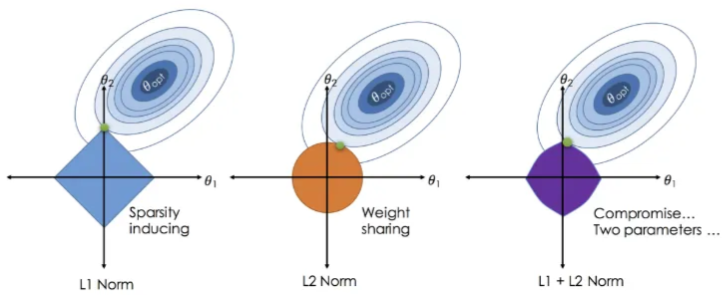
\includegraphics[scale=0.5]{img/regularizers.png}
    \caption{The ridge regularizer draws equipotential circles in our parameter space. The lasso draws a diamond, which tends to give a sparser solution since the loss is most likely to ``touch'' the corners of the contour plots of the regularizer. The elastic net is a linear combination of the ridge and lasso regularizers.} 
    \label{fig:regularizers_visual}
  \end{figure}

  To motivate this even further, let us take the two vectors 
  \begin{align}
    a = \bigg( \frac{1}{\sqrt{d}}, \ldots, \frac{1}{\sqrt{d}} \bigg) \qquad b = ( 1, 0, \ldots, 0)
  \end{align}
  Then the L0, L1, and L2 norms of $a$ are $d, \sqrt{d}, 1$ and those of $b$ are $1, 1, 1$. We want to choose a norm that capture the sparsity of $b$ and distinguishes it from $b$., The L0 norm clearly does this, but the L2 norm does not. The L1 norm is a good compromise between the two. 

  \begin{code}[MWS of Lasso Regression in scikit-learn]
    \noindent\begin{minipage}{.6\textwidth}
    \begin{lstlisting}[]{Code}
      from sklearn.linear_model import Lasso

      X = np.random.randn(10, 5) 
      y = np.random.randn(10)
      # regularization parameter
      model = Lasso(alpha=1e-1)  
      model.fit(X, y) 
      print(model.score(X, y))  
      print(model.intercept_)
      print(model.coef_) 
      print(model.predict(np.array([[1, 2, 3, 4, 5]]))) 
    \end{lstlisting}
    \end{minipage}
    \hfill
    \begin{minipage}{.39\textwidth}
    \begin{lstlisting}[]{Output}
      0.47590269719236045
      -0.8861298412689853
      [0.         0.10767647 0.24172197 0.7427863  0.        ]
      [3.02553422]
      .
      .
      .
      .
      .
    \end{lstlisting}
    \end{minipage}
  \end{code}

\subsection{Bias Variance Tradeoff}

\subsection{Concentration Bounds}

  This now raises the question of how to determine a suitable regularization parameter $\lambda$. The next theorem shows a nice concentration property of the Lasso for bounded covariates. 

  \begin{theorem}[Concentration of Lasso]
    Given $(X, Y)$, assume that $|Y| \leq B$ and $\max_j |X_j| \leq B$. Let 
    \begin{equation}
      \beta^\ast = \argmin_{||\beta||_1 \leq L} r(\beta)
    \end{equation}
    be the best sparse linear predictor in the L1 sense, where $r(\beta) = \mathbb{E}[ (Y - \beta^T X)^2]$. Let our lasso estimator be 
    \begin{equation}
      \hat{\beta} = \argmin_{||\beta||_1 \leq L} \hat{r}(\beta) = \argmin_{||\beta||_1 \leq L} \frac{1}{n} \sum_{i=1}^n (Y_i - \beta^T X_i)^2
    \end{equation}
    which minimizes the empirical risk. Then, with probability at least $1 - \delta$, 
    \begin{equation}
      r(\hat{\beta}) \leq r(\beta^\ast) + \sqrt{\frac{16(L+1)^4 B^2}{n} \log \bigg( \frac{\sqrt{2} d}{\sqrt{\delta}} \bigg)} 
    \end{equation}
  \end{theorem}
  \begin{proof}
    
  \end{proof}

\subsection{Optimization}

  Soft Thresholding and Proximal Gradient Descent
